\section{Application Vulnerabilities} 
\label{sec-vul-study} 
%\setlength{\textfloatsep}{3pt}
%\setlength{\abovecaptionskip}{3pt} \setlength{\belowcaptionskip}{0pt}
%\setlength{\dbltextfloatsep}{3pt}

We studied 12 widely used applications representing different domains, and
ranging in maturity from a few years-old to decades-old.  We studied four
key-value stores (BerkeleyDB~\cite{bdb}, LevelDB~\cite{leveldb},
GDBM~\cite{gdbm}, LMDB~\cite{lmdb}), three relational databases (RDBMS)
(SQLite~\cite{sqlite}, PostgreSQL~\cite{postgres}, HSQLDB~\cite{hsqldb}), two
version control systems (Git~\cite{git}, Mercurial~\cite{mercurial}), two
distributed systems (HDFS~\cite{Shvachko+10-HDFS}, ZooKeeper~\cite{zookeeper})
and a virtualization software (VMWare Player~\cite{vmwareplayer}). We studied two
versions of LevelDB (1.10 and 1.15), since LevelDB's update protocol varies
significantly between the versions.

We first describe the workloads and checkers used in detecting vulnerabilities
(\sref{sec-workload}). We then present an overview of the protocols and
vulnerabilities found in different applications (\sref{sec-case}). In the rest
of this section, we aim to answer the following questions:

\begin{enumerate}[topsep=0pt, itemsep=-1ex, partopsep=1ex, parsep=1ex]
\vspace{-0.03in}
%\item[\textbf{\sref{sec-vuls}.}] How important are the discovered vulnerabilities?% (\sref{sec-vuls})
%\item[\textbf{\sref{sec-patterns}}.] Are there any patterns useful for file system
%design?% (\sref{sec-patterns})
%\item[\textbf{\sref{sec-currentfs}}.] Are vulnerabilities exposed in real file systems?
%\item[\textbf{\sref{sec-twojournal}}.] Can \toolname\ help testing new file system designs?
%
\item How important are discovered vulnerabilities? (\sref{sec-vuls})
\item Are there any patterns among vulnerabilities? (\sref{sec-patterns})
\item How many vulnerabilities are exposed on current file systems? (\sref{sec-currentfs})
\item Can \toolname\ validate new file-system designs? (\sref{sec-twojournal})
\vspace{-0.03in}
\end{enumerate}
%Section~\ref{sec-a} is a brief overview of the workloads and invariants
%verified for each application. Section~\ref{sec-vuls} presents a summary of
%the vulnerabilities found (62), their failure consequences, and their impact
%on top of current file systems. A deeper understanding of the vulnerabilities
%is useful for future file system design, future crash-state exploration tools,
%and for application software design. For this purpose, section~\ref{sec-c}
%analyzes different vulnerabilities according to their type, and
%section~\ref{sec-e} talks about our experience with various aspects of
%application-level consistency. Section~\ref{sec-d} uses the results of our
%study to model a hypothetical file system that maintains application-level
%correctness, while still being efficient.

\subsection{Workloads and Checkers}
\label{sec-workload}
Most applications had configuration options that changed the update protocol or
application crash guarantees. Our workloads tested a total of 36
such configuration options across the 12 applications. 
Our checkers are conceptually simple: they do read operations to verify
workload invariants for that particular configuration, and then try writes to
the datastore. However, some applications do not clearly define their crash
guarantees.  Furthermore, many applications provide users with many manual
recovery methods to be used after a crash. Our checkers invoke all recovery
techniques we are aware of, and are hence complex. 

\textbf{Key-value stores and Relational Databases}. Each workload tested
different parts of the protocol, typically opening a database, and inserting
enough data to trigger checkpoints. The BerkeleyDB checker 
always verifies the database and invokes recovery if needed. The
LevelDB checker always invokes the \smalltt{RepairDB} command. We do not
switch on SQLite options that increase performance by risking correctness atop
specific file systems~\cite{ThanuEtAl13-appconsistency-hotdep}.

% always is dubious: it is different from log recovery (which happens
% automatically), and it is unclear whether the command has to be executed
% after a crash. Furthermore, the recovery command is sensitive to seemingly
% unrelated configuration options. Our checker followed the safest method
% possible (all other methods result in more vulnerabilities): invoke the
% recovery tool with specific configuration parameters.

\textbf{Version Control Systems}. Git's crash guarantees are fuzzy;
mailing-list discussions suggest that Git expects a fully ordered file
system~\cite{git-linus}. Mercurial does not provide \textit{any} guarantees,
but does provide a plethora of manual recovery techniques. Our workloads
add two files to the repository and then commit them. The checker
uses commands like \smalltt{git-log}, \smalltt{git-fsck}, and
\smalltt{git-commit} to verify repostiory state. The checkers remove any
leftover lock files, and perform all documented recovery techniques (except
cloning or restoring a backup).

%The checker verifies
%durability and consistency among outputs of various commands. 

\textbf{Virtualization and Distributed Systems}. The VMWare Player workload
issues writes and flushes from within the guest; the checker repairs the
virtual disk and verifies that flushed writes are durable. HDFS is configured
with replicated metadata and restore enabled. HDFS and ZooKeeper workloads
create a new directory hierarchy; the checker tests that created files (until
the crash) exist.  In ZooKeeper, the checker also verifies that quota and ACL
modifications are consistent.

If \toolname\ finds a vulnerability related to a system call, it does not
search for other vulnerabilities related to the same system call. If the system
call is involved in multiple, logically separate vulnerabilities, this has the
effect of hiding some of the vulnerabilities. Most tested applications,
however, have distinct, independent sets of failures (e.g., \textit{dirstate}
and \textit{repository} corruption in Mercurial, consistency and durability
violation in other applications). We uses different checkers for each type of
corruption, and report vulnerabilities for each checker separately. 

\textbf{Summary}. If application invariants for the tested configuration are
explicitly documented, we consider violating those invariants as failure;
otherwise, \toolname\ considers violating a lay user's expectations as failure.
We are careful about any recovery procedures that need to be followed on a
system crash.  Since it is not possible to detail the exact checkers, we plan
to make the checkers, along with the \toolname\ suite, publicly available for
verification and reuse.

\subsection{Overview}
\label{sec-case}

\begin{figure*}[t] \centering
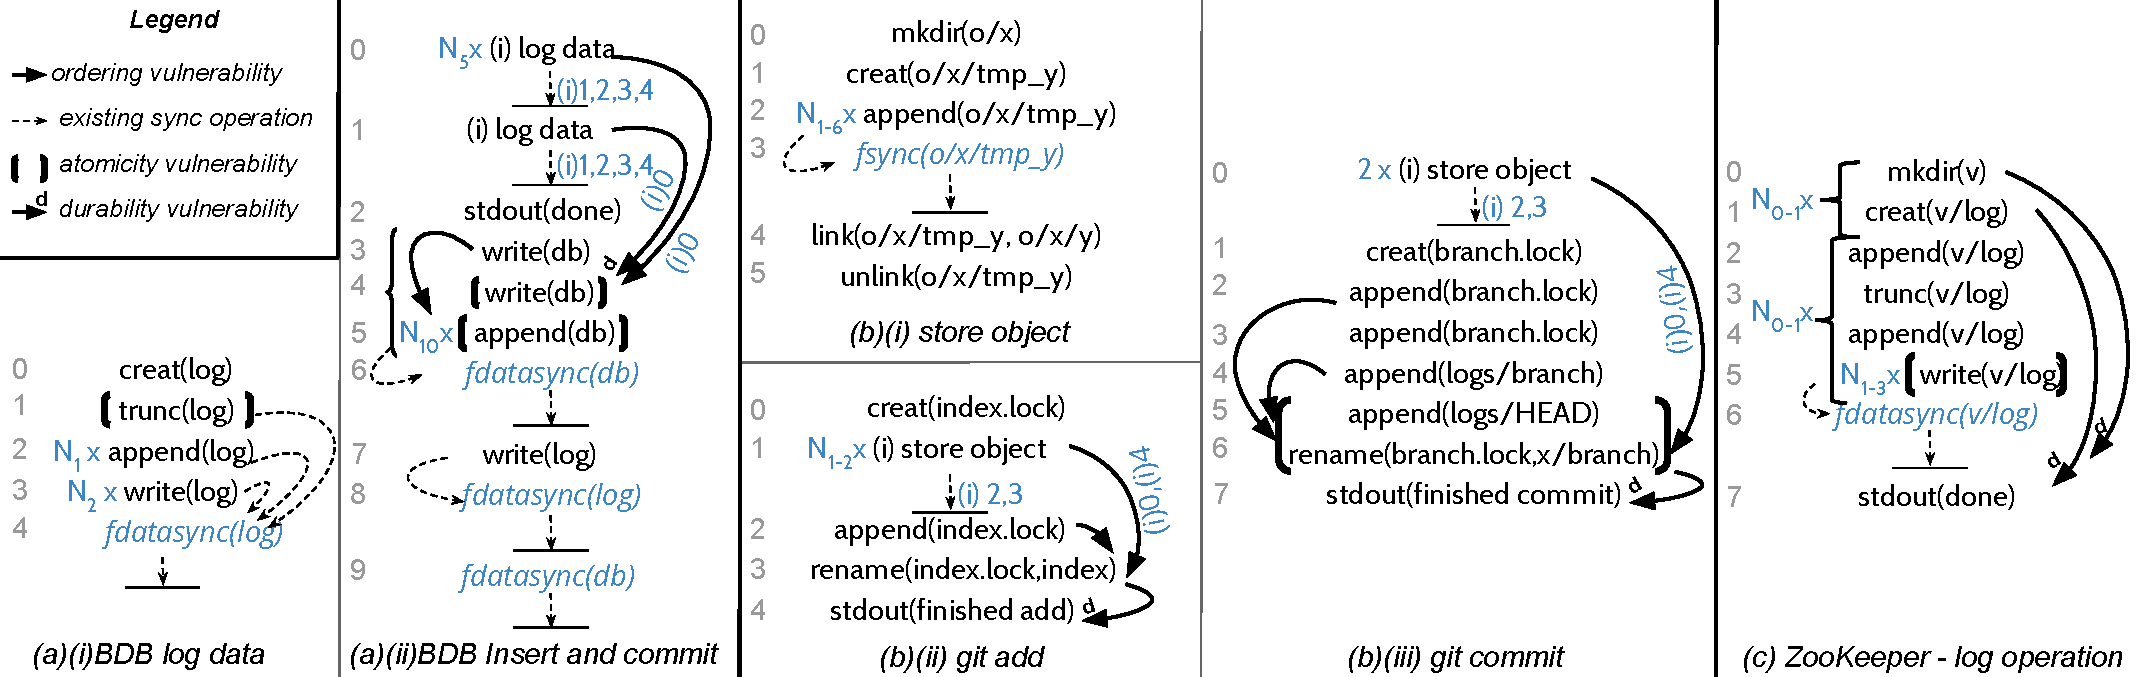
\includegraphics[width=\textwidth]{figs/prot-combined.pdf}
\caption{\label{fig-prot}\textbf{Protocol Diagrams.} {\footnotesize\textit{
(a), (b), and (c) show the modularized update protocol for Git, ZooKeeper, and
BerkeleyDB-BTree respectively. Repeated operations in a protocol
are shown next to each operation, and if the number of repetitions can vary,
the variation is specified. Ordering dependencies are indicated with arrows,
and dependencies between modules are indicated by the numbers on the arrows,
corresponding to line numbers in modules. Dotted, vertical arrows ending at a horizontal
line represent ordering dependencies already enforced using sync operations in the
application. Dark, bold arrows represent new ordering dependencies
discovered; \textbf{d} on the arrow represents a durability requirement.
Operations inside dark brackets must be persisted together atomically.
}}}
\end{figure*}
\newcommand{\refprotbdb}{\ref{fig-prot}(a)}
\newcommand{\refprotgit}{\ref{fig-prot}(b)}
\newcommand{\refprotzookeeper}{\ref{fig-prot}(c)}



We now discuss the logical protocols of the applications we studied. Figure
~\ref{fig-prot} visually represents update protocols from different classes of
applications. The figure shows the logical operations in the protocol
(organized as modules), the ordering ensured by the application via \fsyncSC\
calls, and discovered vulnerabilities.

\subsubsection{Databases and Key-Value Stores}

Most databases use a write-ahead logging technique.  First, the new data is
written to a log. Then, the log is checkpointed or compacted; i.e., the actual
database is carefully overwritten, and the log is deleted.

Figure~\refprotbdb\ show the protocol used by BerkeleyDB, with its BTree
access method. BerkeleyDB adds inserted key-value pairs to the log until it
reaches a threshold, and then switches to a new log.
Figure~\refprotbdb(i) shows the log appends; Figure~\refprotbdb(ii)
shows the complete protocol including checkpointing. During checkpointing,
BerkeleyDB first overwrites the database, then appends to it.
BerkeleyDB marks the end of checkpointing in the log after persisting the
database changes.

In BerkeleyDB and LevelDB-1.15, we found vulnerabilities when initializing or
appending to the log file. For example, a crash during initialization of a
newly created log file might leave the log uninitialized. BerkeleyDB's recovery
code does not handle this situation; the user is unable to open the
database. We also found vulnerabilities during database 
checkpointing. For example, BerkeleyDB does not persist the directory entries of
its logs. A crash during checkpoint might cause the logs to vanish; as a
result, the database might lose data or simply not open.

Some databases follow radically different protocols than write-ahead logging.
For example, LMDB uses shadow-paging (copy-on-write). LMDB requires that the
final pointer update (106 bytes) in the copy-on-write tree to be atomic. HSQLDB
uses a combination of write-ahead logging and update-via-rename, on the same
files, to maintain consistency. The update-via-rename is performed by first
separately deleting the destination file, and then renaming. We found cases
where out-of-order persistence of rename, unlink, or log creation 
causes problems.

\subsubsection{Version Control Systems}

Git and Mercurial maintain meta-information about their repository in the form
of logs. The Git protocol is illustrated in Figure~\refprotgit.
Additionally, Git stores information in the form of object files, which are
never modified; they are created as temporary files, and then linked to their
permanent file names. Git also maintains pointers in separate files, which
point to both the meta-information log and the object files, and are updated
using update-via-rename. Mercurial, on the other hand, uses a journal to
maintain consistency, using update-via-rename only for a few, unimportant
pieces of information.

We found many ordering dependencies in the Git protocol, as shown in
Figure~\refprotgit. This is not surprising, since mailing-list
discussions suggest Git developers expect total ordering from the file system (which no
system provides (\sref{sec-fs-properties})). We also found a Git
vulnerability involving atomicity across multiple system calls; one of the
pointer files being updated (via an append) has to happen atomically with
another file getting updated (via an update-via-rename). In Mercurial, we find
many ordering vulnerabilities for the same reason: the developers have not
designed Mercurial to tolerate out-of-order persistence.

\subsubsection{Virtualization and Distributed Systems} 

Surprisingly, VMWare Player's protocol was simple. VMWare maintains a
static, constant mapping between blocks in the virtual disk, and blocks in the
VMDK file (even for dynamically allocated VMDK files); directly overwriting the VMDK
file maintains consistency (though VMWare does use update-via-rename for some
minor configuration). Both HDFS and ZooKeeper use write ahead logging. 
Figure~\refprotzookeeper\ shows the ZooKeeper logging module. We found that ZooKeeper
does not explicitly persist directory entries of log files; this can lead to lost data.
ZooKeeper also requires the log writes to be atomic.

\if 0
Without \toolname, producing information-rich diagrams such as Figure~\ref{fig-prot}
involves significant manual effort or several rounds of communication with developers.
We inferred several qualitative observations from these studies that helped us 
understand why the current state of application crash vulnerabilities is bad, and
what solutions might be plausible. Section~\ref{sec-discussion} presents our observations.

For example, the primary reason for the HSQLDB
update protocol to be complicated seems to be its layered and modularized architecture.
Git interleaves its concurrency isolation protocol with its update protocol, showing
yet another aspect of complication. While many applications follow the same logical
protocol, the exact implementation varies both by design and by change. As an example,
both VMWare and LMDB sometimes use a separate O\_SYNC descriptor (on an already opened file)
instead of a full \fsyncSC, probably to improve performance. Similarly, a typical way
for logically appending to a file is truncating the file to a bigger size, mapping the truncated
region, and performing memory 
\fi

\subsection{Vulnerabilities Found}
\label{sec-vuls}
\setlength{\tempa}{\tabcolsep}
\setlength{\tabcolsep}{1pt}
\begin{table}[t]
\centering
{\footnotesize
\begin{tabular}{>{\scriptsize}l!{\vrule width 1pt}c|cccc|ccc|cc!{\vrule width 1pt}c|c|c|>{\scriptsize}c@{}!{\vrule width 1pt}>{\bfseries}c}
%\begin{tabular}{p{1.0cm}p{1.0cm}p{1.0cm}p{1.0cm}p{1.0cm}p{1.0cm}p{1.0cm}p{1.0cm}p{1.0cm}p{1.0cm}p{1.0cm}p{1.0cm}p{1.0cm}p{1.0cm}}
\multirow{3}{1cm}{\scriptsize \textbf{Application}} & \multicolumn{10}{c!{\vrule width 1pt}}{{\textbf{Types}}} & \multicolumn{4}{c!{\vrule width 1pt}}{{\textbf{Failure Consequences}}} & \multirow{3}{*}{\rotatebox{90}{{Unique static vulnerabilities~~~}}} \\ \cline{2-11}\cline{12-15}
 & \multirow{2}{*}{\rotatebox{90}{\textbf{Across-syscalls atomicity~~~~}}} & \multicolumn{4}{c|}{{\scriptsize \textbf{Atomicity}}} & \multicolumn{3}{p{0.38cm}|}{\scriptsize\textbf{Orde-ring}} &  \multicolumn{2}{p{0.3cm}!{\vrule width 1pt}}{\scriptsize\textbf{Dura-bility}} & & & & \\ \cline{3-11}
& 
& \rotatebox{90}{{Appends and truncates}}
& \rotatebox{90}{{Multi-block overwrites}}
& \rotatebox{90}{{Sinlgle-block overwrites}}
& \rotatebox{90}{{Renames and unlinks}}
& \rotatebox{90}{{Safe file flush}}
& \rotatebox{90}{{Safe renames}}
& \rotatebox{90}{{Other}}
& \rotatebox{90}{{No commit}}
& \rotatebox{90}{{Losing old commit}}
& \rotatebox{90}{{Silent corruption}}
& \rotatebox{90}{{Data loss}}
& \rotatebox{90}{{Cannot open}}
& \rotatebox{90}{{{\footnotesize Other}}}
& 
\\ \hline
BDB-BTree &   & 2 & 1 &   &   & 1 &  &  & 1 & 1 &  & 2 & 1{\scriptsize $^{\#}$},2 & 1 failed read & 4 \\ \hline
BDB-Hash &   & 2 &   &   &   &  &  &  & 1 & 2 &   & 3 & 1{\scriptsize $^{\#}$},1 &  & 4 \\ \hline
Leveldb1.10  & 1* &   &   &   &   & 2 &  & 2 & 1 & 2 & 6 & 3 &   &  & 7 \\ \hline
Leveldb1.15  &   & 1 &   &   &   &  &  & 3 &   &   & 4 &  &   &  & 4 \\ \hline
LMDB &   &   &   & 1 &   &  &  &  &   &   &   &  &   & read-only open & 1 \\ \hline
GDBM  & 1 &   &   &   & 1 &  &  & 1 & 2 &   &   & 2 & 3 &  & 5 \\ \hline
HSQLDB  &   & 1 &   &   & 2 & 1 &  & 3 & 1 & 2 & 2 & 3 & 5 &  & 10 \\ \hline
Sqlite-Roll &   &   &   &   &   &  &  &  & 1 &   &   & 1 &   &  & 1 \\ \hline
PostgreSQL &  &  &  & 1 &  &  &  &  &  &  &  &  & 1{\scriptsize $^{\#}$} &  & 1 \\ \hline
Git  & 1 &   &   &   & 1 & 2 & 1 & 3 & 1 &   &   & 1 & 5 & 3$^{+}$ & 9 \\ \hline
Mercurial & 4 & 1 &   &   & 1 &  & 1 & 4 & 2 &   &   & 2 & 6 & 7 dirstate fail & 12 \\ \hline
VMWare &   &   &   &   & 1 &  &  &  &   &   &   &  & 1 &  & 1 \\ \hline
HDFS &  &  &  &  & 1 &  &  & 1 &  &  &  &  & 2 &  & 2 \\ \hline
ZooKeeper &  &  &  & 1 &  &  &  & 1 & 2 &  &  & 2 & 2 &  & 4 \\ \hline
Total & \textbf{6} & \textbf{7} & \textbf{1} & \textbf{3} & \textbf{7} & \textbf{6} & \textbf{2} & \textbf{18} & \textbf{12} & \textbf{7} & \textbf{12} & \textbf{19} & \textbf{30} & \textbf{12} & \textbf{65}\\
\end{tabular}
}
\caption{\textbf{Vulnerabilities - Types and Consequences.} \textit{
{\footnotesize
The table shows the discovered static vulnerabilities categorized by the type of persistence property and consequences. The number of unique vulnerabilities for an application can be different from the sum of the categorized vulnerabilities, since the same source code lines can exhibit different behavior. SQLite-WAL is not shown because we did not find any vulnerabilities. \textbf{*} The atomicity vulnerability in Leveldb1.10 corresponds to multiple mmap() writes. \textbf{$^{+}$} There are 2 fsck-only and 1 reflog-only errors in Git. \textbf{{\scriptsize $^{\#}$}} These are known, documented failures.
}
}}
\label{tbl-vuls}
\end{table}
\setlength{\tabcolsep}{\tempa}



\toolname\ revealed \totbugs\ static vulnerabilities in total, corresponding to 162
dynamic vulnerabilities. Altogether, applications failed in more than 4000
crash states. Table~\ref{tbl-vuls} presents statistics for each application,
classifying vulnerabilities based on the affected persistence property and
failure consequence. We reiterate here that \totbugs\ is a conservative
estimate of the number of logical vulnerabilities. Particularly, in
Mercurial, we were unable to correlate system calls with stack traces, since
the application is written in Python; we conservatively associate each type of
system call to one line of source code.

Some application configuration options change the entire update protocol. For
example, the different storage engines provided by BerkeleyDB and SQLite use
different protocols, and consequently have different vulnerabilities.
Table~\ref{tbl-vuls} shows each such configuration separately. Once a storage
engine is selected, other configuration options only changed the application
invariants. With different configurations of the same update protocol, all
vulnerabilities were revealed in the \textit{safest} configuration.
Table~\ref{tbl-vuls}, and the rest of the paper, only show the vulnerabilities
found in the safest configuration; i.e., we do not count separately the same
vulnerabilities from different configurations of the same protocol.

We find many vulnerabilities have severe consequences such as silent data
corruption or data loss.
% We classify vulnerabilities that result in durability
% loss as a separate category since they are affected by persistence properties
% in a different manner from other vulnerabilities.
Table~\ref{tbl-vuls} shows
the vulnerability consequences. Eight applications (and both BerkeleyDB
configurations) are affected by data loss, while two (including both
LevelDB versions) are affected by silent corruption. The \textit{cannot open}
failures include failure to start the server in HDFS and ZooKeeper, and 
preventing the user from running basic commands (e.g., \smalltt{git-log},
\smalltt{git-commit}) in VCS. Many \textit{cannot open} failures are due to
fully corrupted datastores, while a few can be solved by application experts.
Since we carefully integrated documented crash recovery techniques into
our checkers, we believe lay users cannot recover from \textit{cannot open}
failures. We also surveyed if any discovered vulnerabilities are previously known,
or considered inconsequential. Two BerkeleyDB vulnerabilities and the single
PostgreSQL vulnerability are documented; they can be solved only with
non-standard (although simple) recovery techniques. The seven \textit{dirstate
fail} vulnerabilities in Mercurial are separated from \textit{cannot
open} failures since they are less harmful (though frustrating to the lay user).
Although Git's \smalltt{fsck}-only and \smalltt{reflog}-only errors are potentially
dangerous, they do not seem to affect normal usage.

Vulnerabilities exposed by \toolname\ are hard to reproduce without using it,
and thus are difficult to report to application developers. Nevertheless, we
reported five vulnerabilities, one each from HSQLDB, LevelDB-1.10, SQLite,
GDBM, and BerkeleyDB. HSQLDB and LevelDB-1.10 confirmed the vulnerability.
HSQLDB does not intend to fix the vulnerability since they consider it an OS
problem (the vulnerability assumes content-atomic appends). When we reported the
LevelDB vulnerability, a fix was already underway, though not yet available
publicly. SQLite and GDBM developers replied that the expected invariants
(durability) were not guaranteed for our workloads; we attribute both found
vulnerabilities to erratic documentation. BerkeleyDB developers are
investigating our report.

% Rephrase to make this more impressive.
\textbf{Summary}. \toolname\ detected \totbugs\ vulnerabilities in total, with 13
resulting in corruption, 19 in loss of durability, and 31 leading to
inaccessible applications. \toolname\ was able to detect previously known
vulnerabilities. 

\subsection{Common Patterns}
\label{sec-patterns}

We examine vulnerabilities related with different persistence properties. 
Since durability vulnerabilities can result from the violation of any persistence
property, we consider them separately. 

\subsubsection{Atomicity across System Calls} 

GDBM, Mercurial, and Git require atomicity across system calls. However, the vulnerability
consequences seem minor: database inaccessibility in GDBM, dirstate corruption
in Mercurial, and erratic \smalltt{reflog} output in Git.
%In GDBM, a crash during database creation 
%leads to database inaccessibility. In Mercurial, the dirstate is
%corrupted. In Git, \smalltt{reflog} is erratic; while this is potentially 
%dangerous, we believe \smalltt{reflog} is rarely used for serious operations.

LevelDB-1.10 works correctly only if multiple writes to a \smalltt{mmap()}-ed
file are persisted atomically. We believe this particular vulnerability is an
outlier.  LevelDB is logically appending to a log using \smalltt{mmap()}-ed
I/O; the vulnerability is similar to a content-atomic append vulnerability.

\subsubsection{Atomicity within System Calls} 

\textbf{Append atomicity}. Surprisingly, four applications require appends to be
\textit{content-atomic}: the appended portion should contain actual data. The
failure consequences are severe, such as corrupted reads (HSQLDB, BerkeleyDB
and LevelDB-1.15) and repository corruption (Mercurial). Filling the appended
portion with zeros instead of garbage still causes failure; only the current
implementation of delayed allocation (where file size does not increase until
actual content is persisted) works. Most appends do not need to be
\textit{block-atomic}; only Mercurial is affected, and the affected append also
requires content-atomicity. BerkeleyDB requires that newly truncated (expanded)
file regions contain zeroes for correctness.

\textbf{Overwrite atomicity}. LMDB, PostgreSQL, and ZooKeeper require small
writes ($<200$ bytes) to be atomic. The LMDB and PostgreSQL writes happen to
fixed file locations. The PostgreSQL vulnerability is documented. Only
BerkeleyDB requires a two-block write to be atomic; a violation
results in a \textit{cannot open} failure. Interestingly, the BerkeleyDB source
lines issuing the write are also involved in the atomic append vulnerability.

Thus, when compared with append atomicity, multi-block overwrite atomicity
vulnerabilities are strikingly less prevalent. Some of the difference can be
attributed to the persistence model (overwrites are content-atomic), and to some
workloads simply not using overwrites. However, the major cause seems to be the
basic mechanism behind application update protocols: modifications are first
logged, in some form, via appends; logged data is then used to overwrite the
actual data. Applications have careful mechanisms to detect and repair failures
in the actual data, but overlook corruptions of the logged data.

\textbf{Directory operation atomicity}. Given how most file systems provide
atomic directory operations (\sref{sec-fs-properties}), one would expect that
most applications would be vulnerable to such operations not being atomic.
However, we find this is not the case. Databases do not employ atomic renames
extensively; consequently, non-atomic renames only affected two databases (GDBM,
HSQLDB). Git, Mercurial, HDFS, and VMWare Player also use rename sparingly, resulting
in only one rename vulnerability in each application. Non-atomic unlinks 
affect only HSQLDB (which uses unlinks for logically performing renames),
while non-atomic truncates (that reduce file size) do not affect any application.

% We conclude that it is most important for file systems to maintain
% content-atomicity of appends. Individual applications can be easily modified
% if the renames are broken. Breaking the atomicity of other operations each
% affects few applications.

\subsubsection{Ordering between System Calls} 
Applications are extremely vulnerable to system calls being persisted out of
order; we found 25 vulnerabilities. 

%Current file systems that persist system
%calls out of order typically use simple heuristics to prevent dangerous
%application failures. We investigated two persistence properties that have
%been considered in the past by file-system designers.

\textbf{Safe renames}. On file systems with delayed allocation, a common
heuristic to prevent  data loss is to persist all appends to a
file before subsequent renames of the file~\cite{URLmassivefsthread}. We found
that this heuristic only fixes 2 discovered vulnerabilities, 1 each in Git and
Mercurial.  We believe the heuristic is more useful for a different class of
applications (e.g., GNOME applications) than those we study.

\textbf{Safe file flush}. A \fsyncSC\ on a file 
does not guarantee that the file's directory entry is also persisted. Most file systems,
however, persist directory entries that the file is dependent on (e,g.,
directory entries of the file and its parent). We found that this behavior is required
by 4 applications for maintaining even basic consistency. Additionally,
ZooKeeper requires it for durability.

\subsubsection{Durability} 
We found two distinct durability loss scenarios: data is
not committed properly and hence lost; or, data that
\textit{was} correctly committed previously is lost later.

\textbf{Not properly committing data}. We find 12 instances where applications
fail to correctly commit data. Improper commit happens in one of two ways:
applications might simply not \fsyncSC\ written data (e.g., GDBM); applications
might not persist the \creatSC\ or \mkdirSC\ of the file hierarchy containing the
data (e.g., HSQLDB, LevelDB-1.10, ZooKeeper); applications may also fail to
persist a directory operation or a small \writeSC marking transaction completion (e.g.,
\unlinkSC\ in SQLite, \renameSC\ in Git, \writeSC in BerkeleyDB).

\textbf{Losing pre-committed data.} Certain vulnerabilities might result in the
applications losing data that was already committed. We observe 7 such
vulnerabilities, spread across BerkeleyDB, HSQLDB, and LevelDB-1.10. Most were
ordering vulnerabilities, while one depended on atomicity of an append 
(BerkeleyDB). We further analyzed BerkeleyDB to understand the root
cause; under the failing crash states, the \smalltt{DB\_Verify} command does not
detect any inconsistencies, and hence our checker opens the database without
explicitly calling \smalltt{DB\_Recover}. In other databases, though our
checkers always call all available recovery commands, we believe the root cause
is similar to BerkeleyDB: incorrect recovery code.

\if 0
\subsubsection{Manual Testing}

%By default, \toolname\ violates one persistence property at a
%time. We investigated the effect of violating multiple properties
%simultaneously: specifically, atomicity and ordering together.  

\toolname\, by default, only covers crash states corresponding to the
persistence properties in~\sref{sec-pptested}. We hypothesize that more
complicated crash states do not usually reveal more vulnerabilties. To verify
this, we configured \toolname\ to also test for vulnerabilities occurring
because of ordering dependencies between invdividual micro-operations (as
opposed to full system calls). We we only found one instance, in ZooKeeper, of
a new, unique static vulnerability in this testing. The vulnerability is
exposed when a write system call is broken down, and only one part of it
bufferred until another write call is persisted. We also manually looked for
vulnerabilities in suspicious portions of all protocols. This revealed only one
additional vulnerability - in LevelDB-1.10, if two unlinks are not persisted
in-order, but a rename between them is.

%The reason complicated crash states do not reveal more vulnerabilities, is because
%update protocols are conceptually simple. Their exact implementations, which are
%often the reason for vulnerabilities, is affected by the straightforward persistence
%properties in~\sref{sec-pptested}.
\fi

% Rephrase??
\subsubsection{Summary} 

We believe our study offers several insights for file-system
designers. Vulnerabilities involving atomicity of multiple system calls seem to have minor
consequences. We believe that it is sufficient for future file systems to focus
on providing atomicity \textit{within} a system call, and ordering between
system calls. 

Breaking the atomicity of directory operations does not have severe
implications for many applications; this could point to a way to improve
file-system performance. 

Missing \textit{sync} operations are not the only reason for
durability loss -- atomicity and ordering vulnerabilities also lead to data
loss.  Therefore, features such as atomic appends can help prevent data loss.

\subsection{Vulnerabilities On Current File Systems}
\label{sec-currentfs}

\setlength{\tempa}{\tabcolsep}
\setlength{\tabcolsep}{1pt}
\begin{table}[t]
\begin{subtable}[t]{0.27\textwidth}
	{\footnotesize
	\begin{tabular}{>{\scriptsize}l|>{\scriptsize}p{2.94cm}|@{}>{\scriptsize}p{0.38cm}@{}@{}>{\scriptsize}p{0.38cm}@{}@{}>{\scriptsize}p{0.3cm}@{}}
	%\hline
	 & \multirow{2}{3.0cm}{\hspace{1.1cm}\textbf{Ordering}}&\multicolumn{3}{c}{\scriptsize\textbf{Atomicity}}\\ \cline{3-5}
	 &  & \multicolumn{1}{@{}c@{}|}{\scriptsize DO} & \multicolumn{1}{@{}c@{}|}{\scriptsize AG}  & \multicolumn{1}{@{}c@{}}{\scriptsize CA}  \\ \hline
	\rotatebox{90}{\hspace{-0.55cm}ext3-w} & Dir ops and file-size changes ordered among themselves, and before sync operations. & \checkmark & 4K & \fwrong \\ \hline
	\rotatebox{90}{\hspace{-0.70cm}ext3-o} & Dir ops, appends, truncates ordered among themselves. Overwrites before non-overwrites, all before sync. & \checkmark & 4K & \checkmark \\ \hline
	\rotatebox{90}{\hspace{-0.05cm}ext3-j\hspace{0.05cm}} & All operations are ordered. & \checkmark & 4K & \checkmark \\ \hline
	\rotatebox{90}{\hspace{-0.55cm}ext4-o} & Safe rename, safe file flush, directory operations ordered among themselves & \checkmark & 4K & \checkmark \\ \hline
	\rotatebox{90}{\hspace{-0.05cm}btrfs\hspace{0.05cm}} & Safe rename, safe file flush & \checkmark & 4K & \checkmark \\
	\end{tabular}
	}
	\centering
	\footnotesize\textit{(a)}
	\vspace{-0.08in}
    \end{subtable}
    ~~
    \begin{subtable}[t]{0.19\textwidth}
	{\footnotesize
	\begin{tabular}{>{\scriptsize}l|ccccc}
%	\multicolumn{6}{c}{}\\
%	\multicolumn{6}{c}{}\\
	& \rotatebox{90}{\textbf{ext3-w}}
	& \rotatebox{90}{\textbf{ext3-o}}
	& \rotatebox{90}{\textbf{ext3-j}}
	& \rotatebox{90}{\textbf{ext4-o}}
	& \rotatebox{90}{\textbf{btrfs}}
	\\ \hline
	BDB-BTree & 3 & 1 & 1 & 1 & 1 \\ \hline
	BDB-Hash & 4 & 1 & 1 & 1 & 2 \\ \hline
	Leveldb1.10  & 2 & 1 & 1 & 1 & 4 \\ \hline
	Leveldb1.15  & 1 &  &  &  & 3 \\ \hline
	%LMDB &  &  &  &  &  \\ \hline
	GDBM  & 2 & 2 & 1 & 2 & 3 \\ \hline
	Git  & 2 & 2 & 2 & 2 & 5 \\ \hline
	Mercurial & 3 & 2 & 2 & 4 & 6 \\ \hline
	HSQLDB  &  &  &  &  & 4 \\ \hline
	%Sqlite-WAL &  &  &  &  &  \\ \hline
	Sqlite-Roll & 1 & 1 & 1 & 1 & 1 \\ \hline
	%VMWare &  &  &  &  &  \\ \hline
	%PostgreSQL &  &  &  &  &  \\ \hline
	HDFS &  &  &  &  & 1 \\ \hline
	ZooKeeper & 1 & 1 &  & 1 & 1 \\ \hline
	Total & 19 & 11 & 9 & 13 & 31 \\
	\end{tabular}
	}
	\centering
	\footnotesize\textit{(b)}
%	\vspace{1mm}
	\vspace{-0.08in}
    \end{subtable}
    \caption{\label{tbl-fs-impact}\textbf{Vulnerabilities on Current File Systems.} {\footnotesize\textit{
    	(a) describes the simple file system models used.  (b) shows the number of vulnerabilities that occur on current file systems. Applications that do not fail in the considered file systems are omitted. Legend: DO: directory operations. AG: granularity of size-atomicity. CA: Content-Atomicity.  }}}
\end{table}

\setlength{\tabcolsep}{\tempa}

 

We evaluated the occurrence of vulnerabilities in current file systems by
configuring \toolname\ with simple persistence models of the file systems. The
considered persistence models are shown in Table~\ref{tbl-fs-impact}(a).
Table~\ref{tbl-fs-impact}(b) shows the vulnerabilities reported by \toolname\
for each file system.

%Table~\ref{tbl-fs-impact}(b) shows a number of interesting results. 
We make a number of observations based on Table~\ref{tbl-fs-impact}(b). First,
a significant number of vulnerabilities are exposed on \textit{all} examined
file systems.  Second, ext3 in data journaling mode is the safest: the only
vulnerabilities exposed are related to durability and atomicity across system
calls. Third, a large number of
vulnerabilities are exposed on btrfs as it aggressively persists operations out
of order~\cite{btrfs-mason}. 

%\textbf{Summary}. As file systems look to gain performance, it results in additional
%vulnerabilities being exposed. This makes it important to test file-system
%design changes do not affect current applications.

\textbf{Summary}. Application vulnerabilities are exposed on many current file
systems; the vulnerabilities exposed vary based on the file system, thus
testing applications on specific file systems does not work.    

%\textit{Are the vulnerabilities exposed in real file systems?} Yes. However,
%not all of them are exposed.

% LevelDB-1.10's vulnerability atop ext3-ordered corresponds to atomicity
% across memory mapped writes, while

% The vulnerability exposed by both Git and SQLite-Rollback atop ext3-ordered
% are durability violations arising from not calling \fsyncSC\ on directory
% operations. Unless a file system provides synchronous writes, these
% vulnerabilities cannot be prevented from occuring. GDBM's vulnerabilities
% happening atop ext3-ordered mode is different, however, and corresponds to
% appends getting persisted after subsequent overwrites. GDBM's vulnerabilities
% can be tolerated by using the data-journaling mode of ext3.

\subsection{Evaluating New File-System Designs} 
\label{sec-twojournal}

File-system modifications for improving performance have introduced wide-spread
data loss in the past~\cite{URLmassivefsthread}, because of changes to the
file-system persistence model. \toolname\ can be used to verify that such
modifications don't break correctness of existing applications. We describe how
we used \toolname\ to evaluate a hypothetical variant of ext3 (data journaling
mode), \smalltt{ext3-fastfsync}.

Our study shows that ext3 (data journaling mode) is the safest file system;
however, it offers poor performance for many
workloads~\cite{PrabhakaranEtAl05-Usenix}. Specifically, \fsyncSC\
latency is extremely high as ext3 persists \textit{all} previous operations on
\fsyncSC. One way to reduce \fsyncSC\ latency would be to modify ext3 to
persist only the synced file. However, other file systems (e.g,. btrfs) that
have attempted to reduce \fsyncSC\ latency~\cite{LWN1} have resulted in increased
vulnerabilities. Our study suggests a way to reduce \fsyncSC\ latency
\textit{without} introducing additional vulnerabilities. 

Based on our study, we hypothesize that data that is not \textit{synced} need
not be persisted before explicitly synced data for correctness. We design
\smalltt{ext3-fastfsync} to reflect this: \fsyncSC\ on a file $A$ persists only
$A$, while other dirty data and files are still persisted in-order.

We modeled \smalltt{ext3-fastfsync} in \toolname\ by introducing a slight
change in the persistence model of ext3. We changed the ordering dependencies
of synced files and their data: previously, they were ordered after all
previous operations; we changed them to depend on previous syncs and operations
necessary for the file to exist (i.e., safe file flush is obeyed).  The
overwrites of a synced file are ordered among themselves.

\toolname\ verified our hypothesis: \smalltt{ext3-fastfsync} does not expose
any of the observed ordering vulnerabilities on the 12 tested applications.
The design was not meant to fix durability or atomicity across system calls
vulnerabilities, so those vulnerabilities are still reported by \toolname. 

We estimated the performance gain of \smalltt{ext3-fastfsync} using the
following experiment: we first write 250 MB to file $A$, then append a byte to
file $B$ and \fsyncSC\ $B$. When both files are on the same ext3-ordered file
system, \fsyncSC\ takes about 4 seconds.  If the files belong to different
ext3-ordered partitions on the same disk, mimicing the behavior of
\smalltt{ext3-fastfsync}, the \fsyncSC\ takes only 40 ms. The first case is 100
times slower because 250 MB of data is ordered before the single byte that
needs to be persistent.

%Evaluating the new design required less than 50 lines of code. We believe the
%ease of use offered by \toolname\ will allow it to be incorporated into the
%design process of new file systems. % Also, at least one new file system design
% derived from inferences provided by \toolname\ seems interesting.

\textbf{Summary}. \toolname\ helps evaluate the impact of changes to
file-system design on application correctness. Evaluating
\smalltt{ext3-fastfsync} required less than 50 lines of code. 
